\section{Modificaciones de la arquitectura y desarrollo}
\todo[inline]{MEter los resultados y las imágenes aquí? O en la sección de resultados? Podriamos o hacer referencia a esta sección en la de discusión o limitar esta sección a esquemas, código y explicación teórica de que se ha cambiado para luego en la sección de resultados repetir entre comillas los apartados de esta seccion solamente con las gráficas pertinentes (evidentemente comentandolas). Puede que sea mejor opción la segunda}

\subsection{Entrenamiento}
Script de entrenamiento, dataloader, todas las cosas que se han hecho para acelerar el entrenamiento. Hablar de las horas de entrenamiento? Puede que se mezclen cosas con el apartado de metodología?

\subsection{Reducción de tamaño de la entrada}
Para acelerar DPT, lo primero que se modificó fue el tamaño de la entrada. Los resultados de la publicación original calculan la profundidad en el conjunto de evaluación de KITTI con las imágenes en su tamaño original, 1216x352, para reducir el consumo de memoria del modelo durante su entrenamiento, así como acelerar entrenamiento e inferencia, se han añadido dos operaciones de cambio de tamaño: una al principio de la red que reduce el tamaño de las imágenes a 640x192 píxeles, y otra al final de la red que reescala la salida al tamaño original. La primera operación emplea como método de interpolación el algorítmo \texttt{INTER{\_}AREA} de OpenCV, que TODO y está recomendado para reducir el tamaño de imágenes ya que proporciona resultados sin efecto Moire; la operación que amplia la salida al tamaño de la imagen original, por otro lado, emplea interpolación bicúbica, que ofrece los mejores resultados pese a ser más lenta, ya que el tiempo empleado en las operaciones de reescalado es despreciable en comparación con el tiempo de inferencia de la red.

\todo[inline]{Medir el tiempo que está escalando y haciendo inferencia para justificar la frase del final}
\todo[inline]{Hacer una comparación de velocidad de inferencia con la imagen en grande y con la imagen en pequeño}
\todo[inline]{Entrenar un modelo con la imagen grande para ver como afecta? Podría ser solo uno, similar a la prueba que se quiere hacer con el resnet entrenado en imagenet}
\todo[inline]{Explicar inter{\_}area, citarlo? explicar en una nota al pie qué es el efecto moire?}

% https://medium.com/@wenrudong/what-is-opencvs-inter-area-actually-doing-282a626a09b3

\subsection{Número de cabezas}
Hablar del cambio en el número de cabezas
\todo[inline]{Citar y justificar esta dirección de búsqueda con el paper de are 16 heads better than 1}

\subsection{Capas de atención eficiente}
Cambio de las capas, hacer una gráfica midiendo en función del tamaño de la cadena la velocidad en la que pasa por una de estas capas? Puede ser interesante. (Sería para imágenes mayores)

\todo[inline]{Hacer un estudio del incremento de velocidad en función del tamaño de los tokens, es posible que haga falta usar una máquina de Google Cloud para esto, se puede coger una gorda con mucha mucha memoria, habría que incluirla en el apartado de hardware, también se podría usar para el cálculo de el flujo máximo de imagenes (una A100/P100). Se podría usar la misma imagen en teoría, si sale bien mencionarlo también en el apartado de Docker o en el de Google Cloud}

\subsection{Cambio en los hooks del transformer y eliminación de las capas de atención posteriores}

Hablar del cambio en los hooks, en el paper original se valora el cambio de hooks en la etapa convolucional, pero no en el transformer, se estudian 0,1; 2,5; 8,11

Al modificar las capas del transformer de las que se cogen las activaciones para pasarlas a la etapa de fusión convolucional, se abre la posibilidad de eliminar aquellos bloques de atención que ya no se usan. Esta modificación, además de acelerar el entrenamiento e inferencia del modelo, reduce su tamaño considerablemente, tanto a la hora de almacenar sus parámetros como a la hora de cargarlo en memoria para desplegarlo en una aplicación real. En la Figura \ref{fig:attention_block_num}, se puede apreciar la modificación del ViT empleado en DPT: a la izquierda está el encoder tal y como se encuentra en el trabajo de DPT, con los \textit{hooks} en los bloques 8 y 11, sin eliminar ninguno de los parámetros del transformer, y con la inferencia recorriendo los 12 bloques de atención; a la derecha, por otro lado, está una de las opciones valoradas para este hiperparámetro de la arquitectura, donde los hooks se sitúan en la salida de los bloques 0 y 1 del ViT. De esta forma, en el ejemplo, los parámetros a partir del segundo bloque de atención pueden eliminarse ya que la inferencia del modelo solo llega hasta este segundo bloque.

\todo[inline]{Hacer una comparación del tamaño del modelo cuando se eliminan los pesos}
\todo[inline]{Hacer una comparación de los resultados en validación en función de los hooks}
\todo[inline]{Hacer una comparación de la velocidad de inferencia en función de los hooks empleados}
\todo[inline]{Mencionar en la discusión que esto está muy bien porque no están reduciendo la complejidad de la atención, te la estás cargando directamente}
\todo[inline]{Meter el código aquí o una referencia a las partes del código donde se encuentra este cambio?}

\begin{figure}[H]
\centering
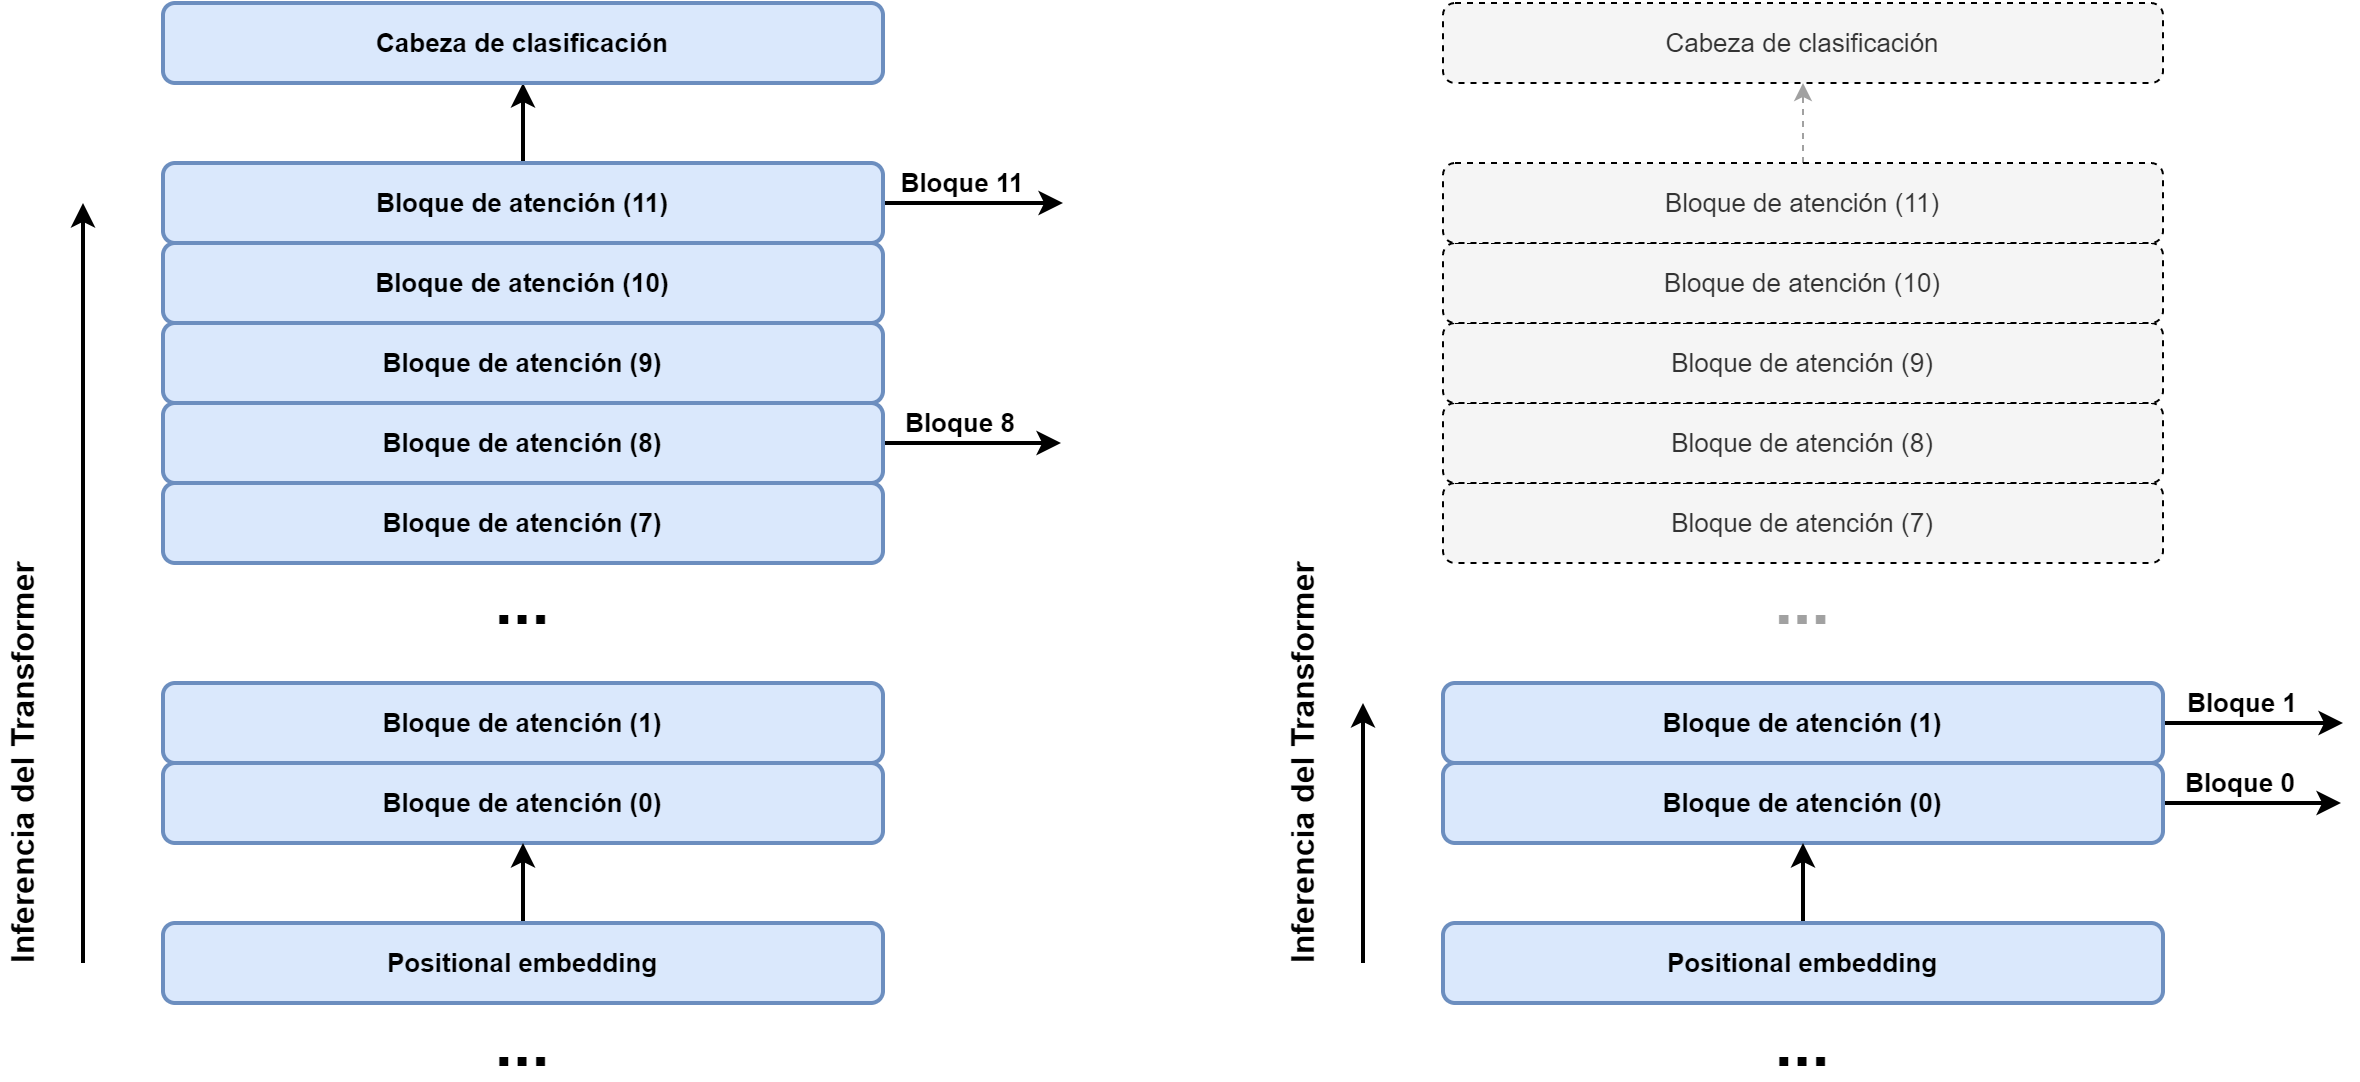
\includegraphics[width=\textwidth]{imagenes/DPT-cambio-bloques-transformer.png}
\caption{Cambio en el número de bloques de atención.}
\label{fig:attention_block_num}
\end{figure}



\begin{figure}[H]
\centering
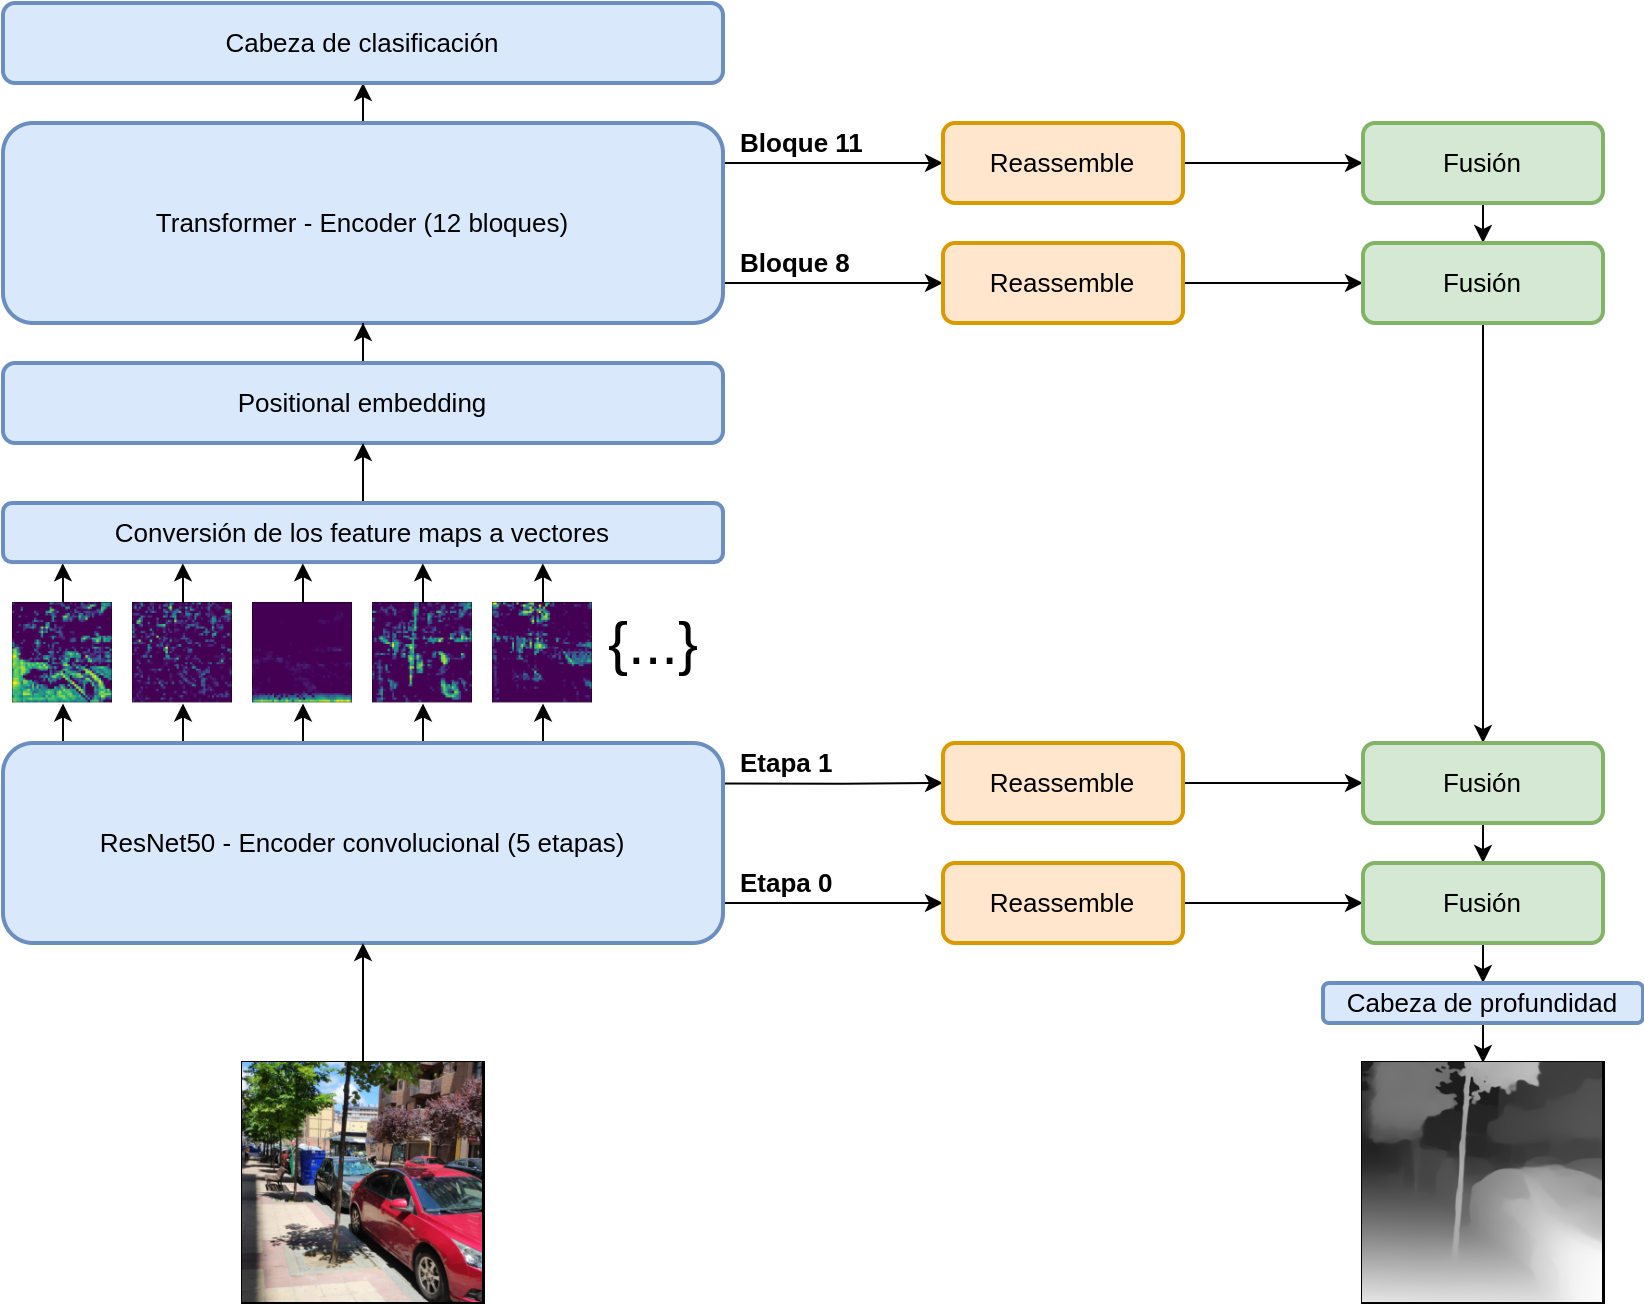
\includegraphics[width=\textwidth]{imagenes/DPT-general.png}
\caption{Arquitectura general DPT.}
\label{fig:dpt-general}
\end{figure}

\begin{figure}[H]
\centering
\includegraphics[width=\textwidth]{imagenes/DPT-modificado-general.png}
\caption{Arquitectura general DPT tras las modificaciones.}
\label{fig:dpt-mod-general}
\end{figure}

\subsection{Cambio del backbone convolucional}
El último cambio estudiado en este proyecto es el del backbone convolucional del Hybrid ViT. En el modulo propuesto en la publicación original, se elige como backbone una ResNet50v2, de la que se extraen las activaciones en los bloques 0 y 1, que tienen un tamaño TODO de 256 y 512, quedando así TODO de tamaños [256, 512, 768, 768]. Por otro lado, la salida de la última capa de la ResNet50v2, es decir, la entrada de los bloques de atención, tiene forma [n, c, h, w], donde n es el número de imágenes en el batch (batch size), c el número de canales (en este caso mapas de características), que son 1024 por como está diseñada la arquitectura, y por último, h y w, que son la altura y anchura de los mapas de características y son iguales a las dimensiones de la imagen de entrada divididas 4 veces entre 2. Después de la ResNet, hay una capa de proyección que no es más que una capa convolucional con kernels de tamaño 1x1 y stride 1x1, con 1024 canales de entrada y 768 canales de salida. Este tipo de capas, realmente son 786 kernels de 1x1x1024, por lo que al convolucionar cada uno de ellos la entrada, se obtienen 768 mapas de características del mismo tamaño que los de la entrada. Los 768 mapas de características resultantes, se aplanan en tensores de forma [n, 768, h/8 * w/8] y se transponen de forma que la entrada sea de tipo [n, t, 768], donde 768 es el tamaño de los tokens de los bloques de atención y t el número de tokens extraidos de la imagen. De esta forma, a mayor tamaño de imagen mayor será el número de tokens, pero la dimensión de estos permanece constante.

\todo[inline]{Hablar de las convoluciones con kernels 1x1 arriba en vez de aquí?}

A modo de ejemplo, supongamos una entrada de una sola imagen de tamaño 384x384: la salida de la ResNet50v2 tendrá la forma [1, 1024, 24, 24]. Esta salida atraviesa la capa de proyección y pasa a tener forma [1, 768, 24, 24]. Estos mapas de características se aplanan en un tensor [1, 768, 576] que se traspone para obtener la forma [1, 576, 768], que equivale a 576 tokens de dimensión 768. Una vez llegados a este punto, el tensor está listo para pasar a los bloques de atención del transformer.

Por otro lado, la arquitectura EfficientNet-B0, alternativa usada en las pruebas de este trabajo, proporciona una salida (antes de la capa de global pooling) de forma [n, c, h, w] donde n vuelve a ser el número de imágenes procesadas en paralelo, el número de mapas de características es en este caso 1280, y la altura y anchura se corresponden con las de las imágenes de entrada divididas 5 veces entre 2. Es decir: [n, 1280, h/16, w/16]. Para poder sustituir el backbone convolucional del Hybrid ViT sin tener que cambiar el tamaño de todas las capas de atención (para poder aprovechar los pesos preentrenados), se sustituye la capa de proyección mencionada en el párrafo superior, que recordemos era una capa convolucional con kernels de tamaño 1x1 por una capa de convolución transpuesta. Esta capa de convolución transpuesta, cumple dos funciones fundamentales: la primera, transforma los 1280 mapas de características en 768; y la segunda, al tener un kernel de tamaño 2x2 y un stride también de 2x2, consigue que las dimensiones de estos mapas de características se multiplen exactamente por 2 en ambas dimensiones, convirtiendo la entrada [n, 1280, h/16, w/16] en [n, 1280, h/8, w/8], que es lo que espera la etapa que aplana los mapas de características y transpone el tensor para obtener de nuevo la entrada preparada para los bloques de atención de forma [n, t, 768] donde t vuelve a ser el número de tokens que pasan al transformer, cada uno de dimensión 768.

\todo[inline]{Explicar bien y añadir en el parrafo de efficientnet el tamaño que tienen los hooks de la red convolucional}
\todo[inline]{Meter alguna imagen para explicar todo este apartado}
\todo[inline]{Decir lo de que se ha modificado la carga de pesos del modelo}
\todo[inline]{Decir (y luego repetir) que efficientnet no está preentrenada en mix y que esto evidentemente afectará a los resultados}


% En los resultados hablar de la distribución de los pesos antes y después de convertir el modelo si es pertinente, hacer una especie de estudio de ablación si se puede entrenar modelos, etc. Puede estar interesante quitar cabezas de atención, quitar bloques de atención, ver como afecta al tamaño dle modelo, su rendimiento (velocidad y métricas)...

\clearpage